\documentclass[lettersize,journal]{IEEEtran}
\usepackage{amsmath,amsfonts}
\usepackage{algorithmic}
\usepackage{array}
\usepackage[caption=false,font=normalsize,labelfont=sf,textfont=sf]{subfig}
\usepackage{textcomp}
\usepackage{stfloats}
\usepackage{url}
\usepackage{verbatim}
\usepackage{graphicx}
\hyphenation{op-tical net-works semi-conduc-tor IEEE-Xplore}
\def\BibTeX{{\rm B\kern-.05em{\sc i\kern-.025em b}\kern-.08em
    T\kern-.1667em\lower.7ex\hbox{E}\kern-.125emX}}
\usepackage{balance}
\usepackage{booktabs}
\usepackage{bm}
\usepackage{bbm}
\usepackage{float}
\usepackage{hyperref}
\usepackage{dsfont}

\makeatletter
\renewcommand{\paragraph}[1]{%
  \vspace{1.5ex}\textbf{#1}\quad
}
\makeatother

\makeatletter
\renewcommand{\thesection}{\arabic{section}}
\renewcommand{\thesubsection}{\thesection.\arabic{subsection}}
\renewcommand{\thesubsubsection}{\thesubsection.\arabic{subsubsection}}
\renewcommand{\@seccntformat}[1]{\csname the#1\endcsname\quad}
\makeatother


\begin{document}
\title{Computer Vision\\ \vspace{.5em} 
\Large Multi-label Image Classification}
\author{Group 25 \\ \vspace{.2em} Riajul Islam, Andreas Calonius Kreth, Christine Midtgaard}

\maketitle

\begin{abstract}
Multi-label image classification presents significant challenges due to sparse labeling, label imbalance, and the complexity inherent in real-world image datasets. This paper explores two state-of-the-art methodologies addressing these issues: Query2Label (Q2L), which utilizes transformer architectures and asymmetric focal loss to effectively manage label imbalance and localize discriminative features, and Multi-label Learning from Single Positive Labels (MLSPL), which adapts loss functions and employs novel regularization techniques for scenarios with extremely limited supervision. Both models are evaluated on the MS-COCO 2014 dataset and results are reported in mean average precision (mAP). Results indicate that Q2L achieves state of the art performance with its two-stage architecture and MLSPL proves robust in a weakly supervised setting, effectively tackling the challenge of sparse annotations. Results from our experiments show that the methods investigated in this project obtain the expected results on the COCO dataset. However, training with ViT architecture backbones on Q2L has shown to be infeasible due to limited memory in our experimental environment, and thus require a setup with increased computational power. Further improvements in multi-label classification models seem likely due to the potential in these architectures and training strategies.
\end{abstract}

\begin{IEEEkeywords}
Multi-label learning, deep learning, computer vision, multi-label
classification, deep learning for MLC, MS-COCO 2014. 

\end{IEEEkeywords}

% ======================== Introduction ========================

\section{Introduction}

Multi-label classification is a supervised classification task in which each instance can be attached with one or more labels. This difference with respect to single-label or multi-class classification, in which each input is assigned a single class, is what fundamentally changes the nature of the problem. In computer vision, images usually have more than one objects or concepts, so multi-label classification is more appropriate for practical applications such as image tagging, autonomous driving \cite{WU2024105189}, and medical diagnosis \cite{ge2018chestxraysclassificationmultilabel}.
However, multi-label classification is not without its hurdles. Firstly, label correlation can lead to performance issues, as labels are not independent — e.g., beach and ocean tend to co-occur. Second, the imbalance among classes is very common in the real-world datasets, i.e. some categories may occur frequently, while some others may rarely appear, resulting in the model biased toward most categories and ignoring the minority ones. Third, sparse labeling or partial supervision is commonly encountered \cite{mlsp}. Full annotation of every image with all the present labels is costly and not always feasible which eventually leads to training data where only a part of the labels are assigned to each image.
In this work, we study solutions to two fundamental challenges of multi-label learning: (i) learning from sparsely annotated data, namely training from a single positive label per image, and (ii) coping with label imbalance while maintaining the capability of feature localization. 

In computer vision problems in general, Transformers have recently shown a huge potential due to retaining rich spatial information when extracting features in contrast to CNNs discarding information in the convolutional feature map. Therefore, we have chosen to analyse a vision Transformer-based model, which achieves state-of-the-art performance. Query2Label (Q2L) utilizes a two-stage system in which firstly the features are extracted using a backbone network, and in the second stage Transformer encoder-decoder layers are leveraged to pool features using label embeddings as queries. The model learns the label embeddings end-to-end to enhance potential and decrease risk of learning spurious correlations. The state-of-the-art performance together with a novel architecture made this model a likely candidate to investigate. 

Multi-Label Learning from Single Positive Labels (MLSPL) provides a framework to tackle the intrinsic nature of the world being multi-label: scenes typically contain several objects. The challenge of assigning labels when information during training is sparse is explored through this model, which incorporates a novel single positive multi-label loss function that jointly trains the image classifier and estimates missing labels during training. This method is interesting as an efficient method of training multi-label classifiers on images with only a single positive label with minimal supervision could reduce costs of annotating datasets unnecessarily and excessive training. A trade-off in reducing resource costs is worthwhile if the drop in performance is tolerable compared to fully annotated datasets. 

We evaluate the proposed models' performance on the MS-COCO 2014 dataset and discuss mean Average Precision (mAP) performance and the capacity for solving the challenges associated with multi-label image classification.

\section{Related Work}
Multi-label learning has become increasingly sought after in the computer vision research community. There have been several work proposed to enhance the model performance in under label sparsity, class imbalance, and noisy annotations. This section considers related work on loss functions, positive-unlabeled learning, partially observed labels, and attention-based architectures.


\paragraph{Loss Functions}
The loss function is a necessary ingredient of any deep learning model to direct how parmeter should be optimized. Binary Cross-Entropy (BCE) is commonly used for multi-label classification as it is designed to deal with multiple binary targets per sample \cite{mlsp,durand2019learningdeepconvnetmultilabel}. However, BCE treat any unobserved label as the negative, and therefore such approach may not always work as expected in the case where supervision is scarce. Various alternative loss functions have been proposed to deal with class imbalance, such as Focal Loss  which falls back on easy negatives and Asymmetric Loss which treats negative as seriously as positive.

\paragraph{Locating areas of interest}
Another challenge of multi-label classification is how to select which areas of an input image are interesting and only selecting said areas. Early methods would find proposed regions of interest and then treat them as a single-label classification problem \cite{HCP}. Often the discovered bounding boxes would be coarse or be contaminated with background information. Later works would correlate regions of interest with semantic labels by using a spatial transformer layer followed by a Long Short-Term Memory subsystem for predictions \cite{ltsm}.


\paragraph{PU learning} 
The concept of learning from partially labeled samples, in which only positive labels are observed while the others are unknown, is from PU learning. A complete collection of PU learning methods and the corresponding discussions can be found in the survey of Bekker and Davis \cite{Bekker_2020}, and the early investigation in text classification is reported in \cite{Li_2003}. The proposed approaches operate under the assumption that the missing labels may not be negative, a particularly relevant assumption to multi-label image problems. Transplanting such ideas to the case of vision tasks, theoretical works and practical models have been proposed that can learn from noisy weak-supervision datasets, as in the the MLSPL framework \cite{mlsp}.


\paragraph{Partially Observed Labels}
In practice, the great Majority of large Datasets are only partially annotated, as full Annotations are often too costly to obtain. Multiple approaches have been proposed to tackle learning from partially observed labels. Heuristic-based approaches \cite{mlsp} minimize annotation effort but add noise and uncertainty. More principled methods, such as ROLE, attempt to predict missing labels in a structured manner. Durand et al. \cite{durand2019learningdeepconvnetmultilabel} also consider partial labels within the context of deep networks and investigate how the right choice of loss function and architecture can alleviate the problem of false negatives.


\paragraph{Attention and Transformer Architectures}
Transformer-based models have also made a recent foray into computer vision after being successful in natural language processing. The Vision Transformer (ViT) by Dosovitskiy et al. \cite{dosovitskiy2021imageworth16x16words}, applies self-attention mechanism to patches of the image, allowing global context modeling with convolutions. Based on this, Q2L \cite{Query2Label} introduces a transformer decoder that attends to feature map grids using label queries. This makes the model to simultaneously learn the label dependencies and make predictions in a more structured manner. Through employing cross-attention between label embeddings and visual features, Q2L circularly learns label correlations and their spatial distributions. These results showcase the capability of transformer model and structured learning techniques to enhance multi-label classification, especially when the real-world constraints of sparse labels and unbalanced datasets are considered.

% ======================== Theoretical Background ========================
\section{Background}
This section provides essential theoretical background related to multi-label classification tasks, particularly focusing on concepts and methods relevant to MLSPL and Q2L.  Beginning with the definition of multi-label learning, followed by deep neural network architectures in multi-label classification. Finally, the contribution of various loss functions to the training of such neural networks is explored, outlining their roles in mitigating issues inherent in multi-label learning, such as label imbalance and incomplete annotation.

\subsection{Multi-Label Learning}
Contrary to binary or multi-class classification where each instance is associated with only one label, multi-label classification allows assigning multiple labels to a single input \cite{mlsp}. Given $K$ categories, an input image $x\in \mathcal{X}$ is associated with a binary vector of labels $y=[y_1,...,y_K]$ from the label space $\mathcal{Y}=\{0,1\}^K$, where $y_k=1$ represents that $k$ is present in $x$ and $y_k=0$ otherwise. The goal is to create a model that outputs the probability of the presence of a category $p=[p_1,...,p_K]$ \cite{mlsp,Query2Label}.

\subsection{Convolutional Neural Networks (CNNs)}
In the field of computer vision, Convolutional Neural Networks (CNNs) have been a dominant approach for image analysis tasks since their introduction \cite{lecun95}. CNNs are designed to recognize patterns in images by applying local filters through convolutional layers, preserving the two dimensional input of an image \cite{zhang2023dive}. CNNs consist of three main types of layers: convolutional layers, pooling layers, and a Fully Connected (FC) layer \cite{asawaCS231n}. Convolutional layers extract spatial features through learnable filters, pooling layers reduce dimensionality and summarise information, while the fully connected layer at the end interpret the features to perform the classification. Thus, CNNs play a great role in encoding the visual content necessary for classification tasks in both fully and partially labeled multi-label settings, and functions as a backbone architecture in both MLSPL and Q2L.

\subsection{Transformer Architectures}
\label{sec:transformers}
Transformers, introduced by Vaswani et al. \cite{vaswani2023attentionneed}, are a type of neural network architecture initially developed to model long-range dependencies in sequence data. They achieve this using attention and self-attention mechanisms, which enables the model to have a long-term memory of inputs, and dynamically weigh the importance of each element in the input sequence. Originally, transformer-based models was mainly delevoped for natural language processing tasks, but the introduction of the Vision Transformer (ViT) by Dosovitskiy et al. \cite{dosovitskiy2021imageworth16x16words}, transformers have been widely used for computer vision tasks. The following describes the mechanisms of the Transformer, which is a crucial component of the Q2L solution.


\paragraph{Architecture}
The original transformer consists of an encoder-decoder structure. Both encoder and decoder are made of a stack of identical layers, where encoder layers contain a multi-head self-attention mechanism followed by a position-wise feed-forward network. In addition, decoder layers consists of an encoder-decoder attention layer, as illustrated in Figure~\ref{fig:encoder_decoder}. The transfomer decoder is of interest, as the authors of \cite{Query2Label} use them to extract features and automatically learn label embedding, as described in section \ref{sec:q2l_method}.

\begin{figure}[t]
    \centering
    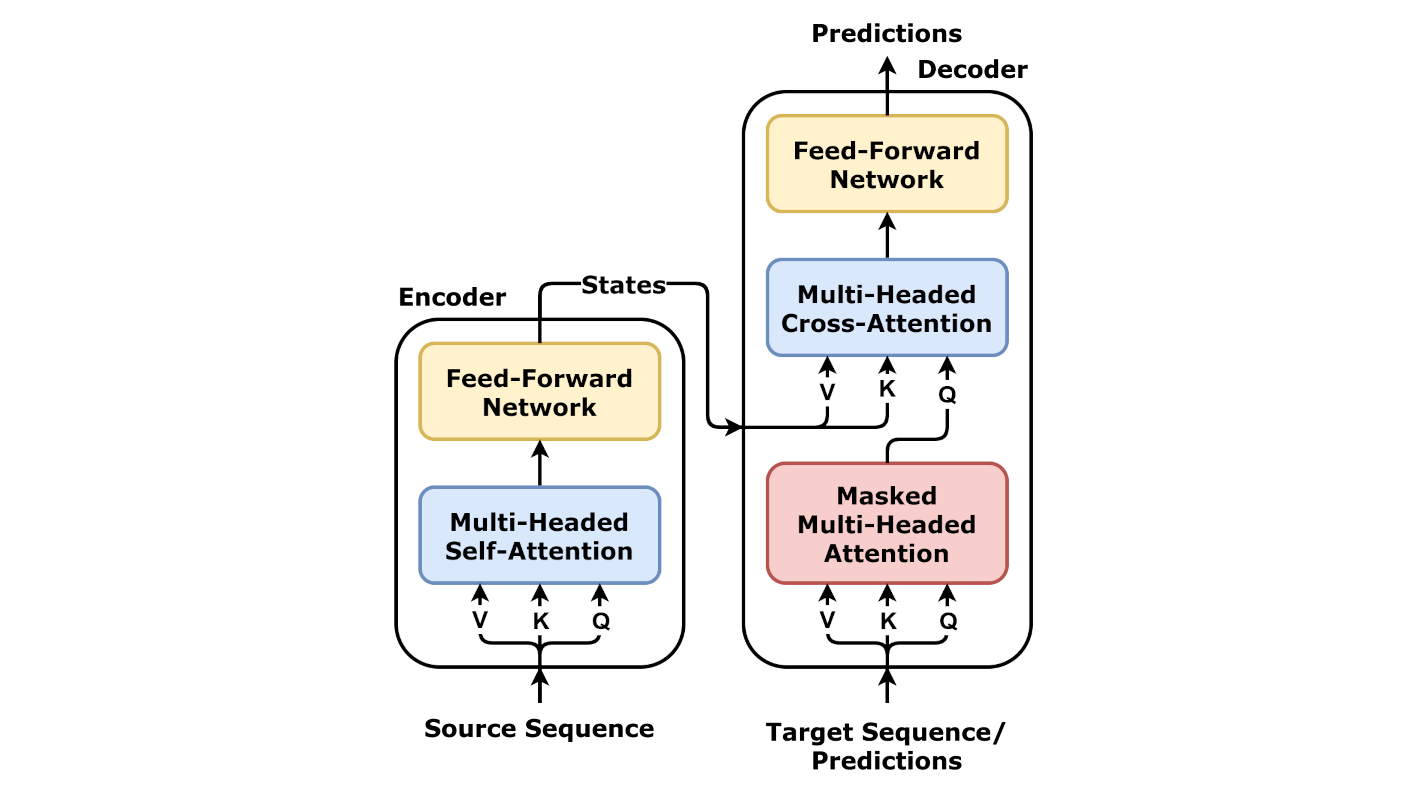
\includegraphics[width=\linewidth]{images/Transformer,_one_encoder-decoder_block.png}
    \caption{Simple Encoder-Decoder. Figure from \cite{godoy_dl_visuals}.}
    \label{fig:encoder_decoder}
\end{figure}

\paragraph{Attention}
The core principle of the transformer architecture is the attention mechanism, which allows the model to attend to all posistions in an input sequence when processing each element. Thus alloowing the model to weigh the relevance of different posistions in a sequence. Given a query and a set of key-value pairs, the attention function computes a weighted sum of the values, where the weights are determined by similarities between the query and the keys.

\paragraph{Self-Attention}
The transformer model uses self-attention by relating every element in the input sequence to every other element. The attention function is a function that maps a query and a set of key-value pairs to an output. The scaled dot-product self-attention is defined as:

\begin{equation}
    \text{Attention}(Q,K,V) = \text{softmax}\left(\frac{QK^T}{\sqrt{d_k}}\right)V
\end{equation}

\noindent where $Q$, $K$, $V$, are the query, key, and value vectors, and $d_k$ is the dimension of the key vectors and serves as a scaling factor \cite{vaswani2023attentionneed}. 

\paragraph{Multi-Head Attention}
The transformer applies multiple attention functions in parallel, allowing the model to attend to information from different parts of the sequence. The embedding is split into multiple heads, perform attention for each, and then concatenate them back together, defined as:

\begin{equation}
    \label{eq:multihead}
    \text{MultiHead}(Q,K,V) = \text{Concat}(\text{head}_1, ..., \text{head}_h)W^O
\end{equation}
    
\noindent where each head is computed as:

\begin{equation}
    \text{head}_i = \text{Attention}(QW^Q_i, KW^K_i, VW^V_i)
\end{equation}

\noindent with projection matrices $W_i^Q$, $W_i^K$, $W_i^V$, and $W_i^O$.

\paragraph{Cross-Attention}
Contrary to self-attention, where queries, keys, and values are generated from the same input, cross-attention is a mechanisn where queries come from one source, and the keys and values come fron another. This mechanism allows the model to relate elements from one input to relevant parts of another input. The authours of Q2L \cite{Query2Label} make use of this mechanism, where label embeddings (queries) attend to spatial image features (key-value pairs).



\paragraph{Feed-Forward Networks and Positional Encoding}
Each layer in the Transformer also includes a fully connected feed-forward network (FNN) applied to each position \cite{vaswani2023attentionneed}. To compensate for the lack of order in the input sequence, sinusoidal positional encodings are added to the input embeddings. These encodings allow the model to distinguish the order of elements in the sequence using functions of varying frequencies. The FNN is defined as:

\begin{equation}
    \label{eq:ffn}
    \text{FFN}(x) = \max(0, xW_1 + b_1)W_2 + b_2\text{,}
\end{equation}

where $x$ is the input vector, $W_1$ and $b_1$ are the weight and bias of the first layer, $\max(0,\cdot)$ is the ReLU activation function, and $W_1$ and $b_1$ are the weight and bias of the second layer

\paragraph{Vision Transformers (ViTs)}
The Vision Transformer (ViT), introduced by Dosovitskiy et al. \cite{dosovitskiy2021imageworth16x16words}, is a model for image classification that leverages the transformer architecture: the self-attention mechanism of transformers that allows the model to selectively weigh the significance of each part of the input, and positional embeddings that represent the order of tokens in a sequence. In ViTs, images are represented as sequences, where the label function as a learnable token for classification. The input image is divided into a sequence of patches that are flattened and linearly embedded into a vector. The spatial information is preserved by adding positional encodings to the embeddings. The resulting sequence is fed into a transformer decoder identical to that introduced in \cite{vaswani2023attentionneed} to model global relations for classification.

\subsection{Loss Functions}
Loss functions are a fundamental component in deep learning as they serve as a measure of how much the model predictions deviate from the ground truth, guiding optimization of the network \cite{zhang2023dive}. The goal of optimization is to minimize the loss. In the context of multi-label learning, each instance can belong to multiple classes simumtaneously, and selecting an appropriate loss function is crucial. This section aims to decribe different loss functions employed in multi-label classification, and how they can be used to solve common issues in multi-label learning.

\paragraph{Binary Cross-Entropy (BCE)}
Due to its effectiveness in handling binary decisions for each class, a common choice of loss function for multi-label classification is the The Binary Cross-Entropy (BCE) loss \cite{mlsp,durand2019learningdeepconvnetmultilabel,nayan2024binary}. In binary classification, the goal is to classify data as either positive or negative, represented as 0 or 1. The output of the model is a probability score between 0 and 1, indicating the probability of the input belonging to the positive class \cite{nayan2024binary}.

The BCE loss for multi-label classification is given by:

\begin{equation}
\begin{aligned}
\mathcal{L}_{\text{BCE}} = -\frac{1}{K} \sum_{i=1}^{K} \bigl[ &y_i\log(p_i) \\
+ &(1-y_i)\log(1 - p_i) \bigr]
\end{aligned}
\end{equation}

\noindent where $K$ is the number of categories, $y_i\in[0,1]$ is the binary label, and $p_i$ is the predicted probability.

Due to its popularity in multi-class classification the BCE loss is used as a benchmark for model performance in \cite{mlsp}. However, BCE loss can be sensitive to class imbalance, where some classes appear more often than others. In this case, the model tends to focus on the majority class and perform poorly on the minority class. Several solutions to this issue have been proposed, where the authors of Q2L address this by incorporating asymmetric focal loss, described later in section~\ref{sec:afl}. 


\paragraph{Loss Functions for the Partially Observed Labels Setting}
BCE assumes that each training example indicates the presence or absence of each class, e.i. the example is fully observable. In real-world multi-label datasets, it is often infeasible to annotate all relevant labels for each image, resulting in only partially observed labels. In the case where labels are only partially observed, the assumption of full negative labeling in BCE can lead to false negatives during training, degrading model performance \cite{mlsp}. 

To address this issue, several loss functions have been proposed to handle partial supervision \cite{mlsp}. In this project, we explore the case of minimal supervision: the single positive label setting, where only one relevant class label is observed per image and the rest are unannotated. The authors of \cite{mlsp} propose Expected Positive Regularization (EPR) and Regularized Online Label Estimation (ROLE) as solutions, described in the following.

\paragraph{Expected Positive Regularization (EPR)}
Assuming that unobserved labels are negative leads to the BCE loss for the positive only case:

\begin{equation}
    \mathcal{L}_{BCE}^+(\mathbf{f}_n,\mathbf{z}_n) = - \sum_{i=1}^{K}\mathds{1}_{[z_{ni}=1]}\log(f_{ni})
\end{equation}

\noindent where $\mathbf{f}_n\in[0,1]^K$ denotes the predicted probabilities for sample $n$, $f_{ni}$ is the probability for class $i$, $\mathbf{z}_n\in\{0,1\}^K$  is the observed label vector, and $\mathds{1}_{[z_{ni}=1]}$ is an indicator function selecting the observed class. However, this predicts all labels as positive. The solution to this is the introduction of a regularization term that contains a domain knowledge. They define a scalar $\kappa$, which is the expected number of positives per image, and an estimated average number of predicted positves $\hat{\kappa}(\mathbf{F}_B)$ from batch predictions, where $\mathbf{F}_B = [f_{ni}]_{n\in B,i\in\{1,...,L\}}$ is defined to be the predictions $f_{ni}\in[0,1]$ for every image in a batch $B\subset \{1,...,N\}$. A regularization term at batch level is introduced to penalize deviations from $\kappa$:

\begin{equation}
    R_\kappa(\mathbf{F}_B) = \left(\frac{\hat{\kappa}(\mathbf{F}_B)-\kappa}{K}\right)^2
\end{equation}

\noindent The overall loss is:

\begin{equation}
    \label{eq:epr}
    \mathcal{L}_{EPR}(\mathbf{F}_B,\mathbf{Z}_B) = \frac{1}{|B|}\sum_{n\in B}\mathcal{L}_{BCE}^+(\mathbf{f}_n,\mathbf{z}_n)+\lambda R_\kappa(\mathbf{F}_B)\text{,}
\end{equation}

\noindent where $\lambda$ is a hyperparameter.


\paragraph{Regularized Online Label Estimation (ROLE)}
The authors of \cite{mlsp} report that $\mathcal{L}_{EPR}$ does not yield satisfactory results, and thus propose a combination of $\mathcal{L}_{EPR}$ and a label estimator module that maintains online estimates of the missing labels during training, called Regularized Online Label Estimation (ROLE). This method jointly trains the image classifier and a label estimator subject to constraints imposed by $\mathcal{L}_{EPR}$. This maintains soft estimates of the full label vector during training, resulting in ROLE assuming unobserved labels to have a probability between 1 and 0. For a batch $B$, let $\mathbf{\tilde{Y}}\in[0,1]^{N\times K}$ represent the estimated labels, and $\mathbf{F}\in[0,1]^{N\times K}$ represent the matrix of classifier predictions. The goal is to jointly train the label estimator $g(\cdot;\phi)$ and the image classifier $f(\cdot;\theta)$. An intermediate loss is defined as:

\begin{equation}
    \label{eq:intermediate}
    \begin{aligned}
        \mathcal{L}'(\mathbf{F}_B,\tilde{\mathbf{Y}}_B) &= \frac{1}{|B|}\sum_{n\in B} \mathcal{L}_{BCE}(\mathbf{f}_n,\text{sg}(\tilde{\mathbf{y}}_n)) \\
        &+ \mathcal{L}_{EPR}(\mathbf{F}_B,\mathbf{Z}_B)\text{,}
    \end{aligned}
\end{equation}

\noindent where $\tilde{\mathbf{Y}}_B\in [0,1]^{N\times K}$ is the matrix of estimated label vectors, $\tilde{\mathbf{y}}_n$ is the estimate for image $n$, and $\text{sg}$ is a stop-gradient. This loss is used to update $\theta$ while keeping $\phi$ fixed. By switching the arguments in Eq.~\ref{eq:intermediate}, $\phi$ is updated while keeping $\theta$ fixed. This leads to the final ROLE loss, given by:

\begin{equation}
    \label{eq:role}
    \mathcal{L}_{ROLE}(\mathbf{F}_B, \mathbf{\tilde{Y}}_B) = \frac{\mathcal{L}'(\mathbf{F}_B)|\mathbf{\tilde{Y}}+\mathcal{L}'(\mathbf{\tilde{Y}}|\mathbf{F}_B)}{2}
\end{equation}

\noindent where both $\mathbf{F}_B$ and $\tilde{\mathbf{Y}}_B$ are updated simultaneously.

\paragraph{Asymmetric focal Loss}
\label{sec:afl}
A simplified version of asymmetric loss function is used by the authors of \cite{Query2Label}. Asymmetric loss is a version of focal loss but with $\gamma$ taking on the value of 0 and 1 for positive and negative values respectively. This loss function effectively addresses the sample imbalance problem by making a distinction between negatives and positives, and focusing on the rarer positive labels while down-weighing the negative samples to prevent them taking over during training. For each training sample the loss is calculated using the following asymmetric focal loss function:

\begin{equation}
    \mathcal{L} = \frac{1}{K} \sum_{k=1}^{K}
\begin{cases}
(1 - p_k)^{\gamma^+} \log(p_k), & \text{if } y_k = 1 \\
(p_k)^{\gamma^-} \log(1 - p_k), & \text{if } y_k = 0
\end{cases}
\end{equation}

\noindent where $y_k$ is a binary indicator of whether sample $x$ contains label $k$. This loss is averaged over the entire data set to calculate the total loss. 

% ======================== Methodology ========================

\section{Method}
We chose to investigate the method proposed in MLSPL as the method for addressing sparse label annotation, and Q2L as the method addressing feature localization. The MS-COCO 2014 was chosen as the multi-label classification becnhmark, as it is widely used in the multi-label learning field. Results are reported in mean Average Precision (mAP). In the following section, the rationale behind the chosen methods is outlined, and how each method aims to solve the multi-label learning challenges.


\subsection{Query2Label: A Simple Transformer Way to Multi-Label Classification}
\label{sec:q2l_method}
We selected Q2L \cite{Query2Label} due to both its novel use of transformer architectures in addressing the challenge of localizing discriminative features in multi-label classification, and its reported state-of-the-art results on the COCO dataset. In contrast to CNN-based methods, Q2L models spatial regions of interest through a query-based attention mechanism. This allows the model to effectively extract features, even when multiple objects of varying sizes exists in a single image \cite{Query2Label}.

\begin{figure}[t]
    \centering
    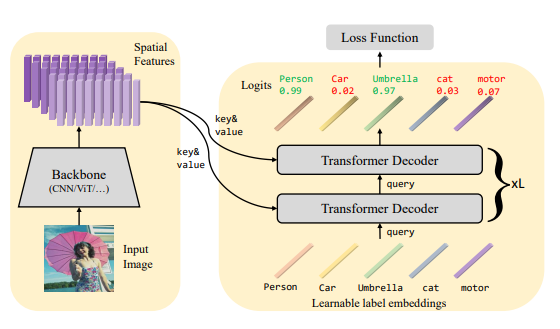
\includegraphics[width=.8\linewidth]{images/q2l_framework.PNG}
    \caption{Query2Label framework.}
    \label{fig:q2l_framework}
\end{figure}

% The label class is treated as a query in the Transformer decoder and the multi-head cross-attention module pools related features to classify them. The averaging of the different heads' attention maps for the label “person” can be seen in the picture below to the right. It would seem that using 3 heads is sufficient for the classification of this specific label as head-2 is not utilized. 

% \begin{figure}[t]
%     \centering
%     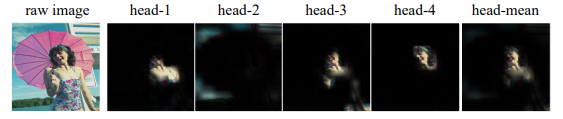
\includegraphics[width=.8\linewidth]{images/q2l_mha.PNG}
%     \caption{Visualization of multi-head attention maps for the target label \textit{person}.}
%     \label{fig:q2l_mha}
% \end{figure}

The Q2L framework consists of two stages. In the first stage, a bockbone network extracts spatial features from an input image. The backbone network can be any architecture, and the authors of Q2L report the performance of various backbone architectures combined with the Q2L method. In the second stage, multiple Transformer decoder layers are implemented (see Section~\ref{sec:transformers}), using label embeddings as queries to check if each label exists. One Transformer encoder layer and two Transformer decoder layers handle feature updates. The transformer encoder layer enhances the global feature context, which makes for better feature representation. The label embedding is compared with features for at each spatial location in order to make attention-maps. Prediction of the existence of any label happens by performing multi-head cross-attention to pool features adaptively (by combining the spatial features based on attention maps) and then doing classification (prediction) based on the pooled features. A linear projection layer is present after the transformer decoder layers, which predicts the logits for each class. In other words, given an input image $x\in \mathbb{R}^{H_0\times W_0\times 3}$ we extract the spatial features $\mathcal{F}_0\in \mathbb{R}^{H_0\times W_0\times d_0}$ where $H_0 \times W_0$ denotes the height and weight of the input image, $H \times W$ represents the height and weight of the feature map and $d_0$ represents the dimension of features. A linear projection layer projects the features from $d_0$ to $d$ to match the query dimension in the second stage to reshape the features into 
The query updating then happens as the label embeddings is used as query: 
$K$ is the number of categories. The queries are updated through a self-attention, a cross-attention and then a feed-forward network, where the following output of each update is given as:

\begin{equation}
    \begin{aligned}
    \text{self-attn:} \quad & Q^{(1)}_i = \text{MultiHead}(\tilde{Q}_{i-1}, \tilde{Q}_{i-1}, \tilde{Q}_{i-1}) \\
    \text{cross-attn:} \quad & Q^{(2)}_i = \text{MultiHead}(\tilde{Q}^{(1)}_i, \tilde{F}, F) \\
    \text{FFN:} \quad & Q_i = \text{FFN}(Q^{(2)}_i)
    \end{aligned}
\end{equation}

Where $\text{MultiHead(query, key, value)}$ is the same as Eq.~\ref{eq:multihead} and $\text{FFN}(x)$ is the same as Eq.~\ref{eq:ffn}. Tilde means the original vectors modified by factoring in position encodings. Additionally, class imbalance is mitigated by applying asymmetric focal loss (Section \ref{sec:afl}) as the chosen loss function for optimization.

The transformer model solves a crucial challenge, which is the need to extract local discriminative features and do this adaptively for different labels. Unlike using the global average-pooled feature map from the final layer of a CNN directly for binary classification, the built in cross-attention module retains rich information when extracting features. Similarities of a given query and extracted spatial features are represented in the mean of each head's cross-attention map as seen on Figure \ref{fig:q2l_attention}.

\begin{figure}[t]
    \centering
    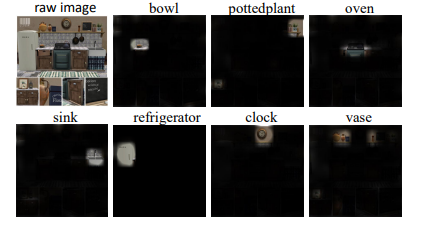
\includegraphics[width=.8\linewidth]{images/q2l_attention.PNG}
    \caption{Visualization of cross-attention maps. Figure from \cite{Query2Label}. }
    \label{fig:q2l_attention}
\end{figure}

As mentioned earlier, the backbone network can be arbitrary. In this project, we replicate the experiments on the following: ResNet-101 with two resolutions ($448\times 448$ and $576\times 576$), TresNetL, TresNetL(22k), Swin-L(22k), and CvT-w24(22k). The results from our experiments can be seen in Table~\ref{tab:q2l_map_comparison}.

\subsection{Multi-Label Learning from Single Positive Labels}
We chose to investigate the method proposed my MLSPL as the solution to the challenge of sparse annotation, a common problem in multi-label classification tasks \cite{mlsp}. The MLSPL framework is designed to learn from the case of minimal supervision: only one positive label per image. This approach reports results of up to $88.2\%$ on the VOC12 dataset, and $69.0$ on the COCO dataset, and thus demonstrates potential to reduce annotation cost significantly.

The authors' solution to this problem lies in the design of the loss function, which combines two key techniques: Expected Positive Regularization (EPR) and Regularized Online Label Estimation (ROLE).

Expected Positive Regularization (EPR) (Eq.~\ref{eq:epr}) introduces a soft constraint on how many positive labels the model should predict per image. This is implemented by penalizing the difference between the predicted number of positives $\hat{k}$ and the an already defined value $k$, thereby avoiding the predicting all labels as postive \cite{mlsp}. ROLE (Eq.~\ref{eq:role}) builds upon EPR by jointly training an image classifier and a label estimator. The label estimator maintains soft predictions for all unobserved labels, and the classifier is trained on a combination of observed and estimated labels. This framework allows the model to recover many of the positive labels.

\begin{figure}[t]
    \centering
    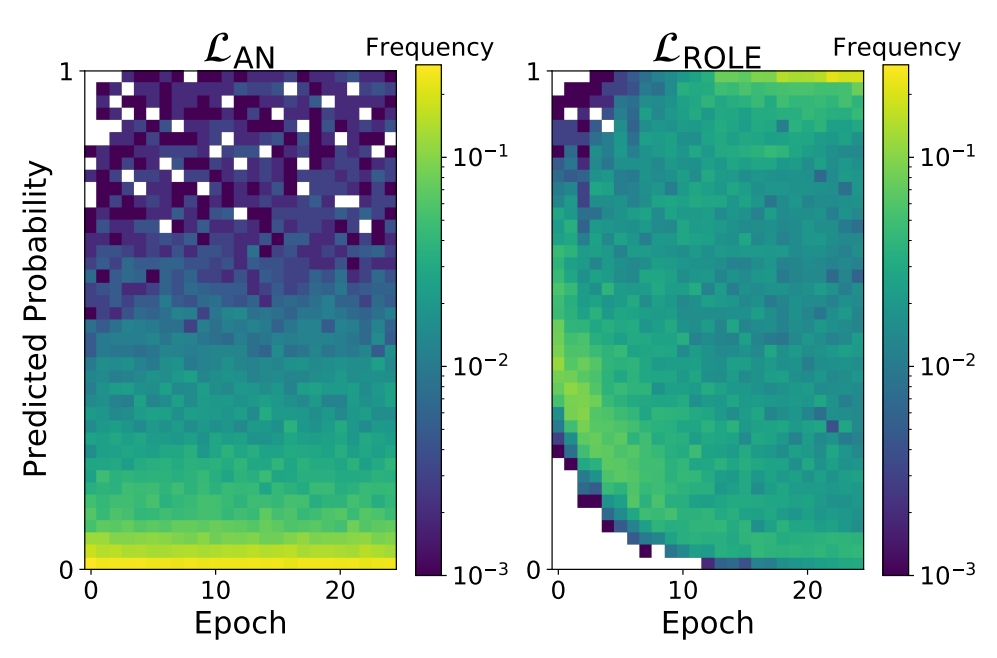
\includegraphics[width=.8\linewidth]{images/mlsp_fig2.png}
    \caption{The distribution of predicted probabilities for unobserved positives when training with a single positive per image for COCO. Figure from \cite{mlsp}.}
    \label{fig:mlsp_fig2}
\end{figure}

The effectiveness of ROLE in recovering unobserved labels is illustrated in Figure~\ref{fig:mlsp_fig2}. 

In replicating the findings from MLSPL, we chose to focus on the performance of $\mathcal{L}_{ROLE}$ on the COCO dataset trained on the linear classifier with fixed features, and the fine-tuned network. In both cases, the backbone is an ImageNet pretrained ResNet-50. Results from our experiments can be seen in Table~\ref{tab:MLSPL_map_comparison}.

% ======================== Experimental Setup  ========================

\section{Experiments}
All experiments were conducted on a cluster with access to two NVIDIA GeForce RTX 3060 GPU (12 GB VRAM). The cluster was equipped with Ubuntu 22.04.5 LTS.

\subsection{Dataset}
The MS-COCO 2014 \cite{coco14} dataset is used as a benchmark for evaluation both Q2L and MLSPL. MS-COCO (Microsoft Common Objects in Context) is a large-scale dataset commonly used for object detection, segmentation, and multi-label image classification. COCO consists of 82,081 training images and 80 classes, and a validation set of 40,137 images. Examples from the COCO dataset can be seen in Figure~\ref{fig:coco-examples}.

\begin{figure}[t]
    \centering
    \includegraphics[width=.8\linewidth]{images/coco_grid.png}
    \caption{Examples from the MS-COCO 2014 training set, resized to $448 \times 448$ pixels.}
    \label{fig:coco-examples}
\end{figure}

\subsection{Evaluation Metrics}
To asses model performance, we adopt mean Average Precision (mAP), a standard metric widely reported in multi-label classification tasks as it is used to analyze the performance on object detection and segmentation. Both Q2L and MLSPL report results in terms of mAP. 

\subsection{Query2Label}
All Q2L experiments were conducted using Python 3.7.3 with PyTorch 1.9.0 and Torchvision 0.10.0, compiled with CUDA 11.1. Due to compatibility issues with the \texttt{inplace\_abn} dependency required by TResNet backbones, we rebuilt the extension from source using commit \texttt{938ffd2} to ensure compatibility with our environment.

Additionally, we encountered a missing dependency for RandAugment, which was not included in the original repository. To address this, we manually added the augmentations.py file from the pytorch-randaugment implementation\footnote{\url{https://github.com/ildoonet/pytorch-randaugment}} and modified the import in get\_dataset.py to use a local version: from .augmentations import RandAugment. We also replaced the default RandAugment() instantiation with RandAugment(n=2, m=9) to explicitly set the parameters. While a similar implementation exists in the torchvision.transforms module\footnote{\url{https://pytorch.org/vision/main/generated/torchvision.transforms.RandAugment.html}}, it is incompatible with the version of torchvision used in this project.

\paragraph{Data preparation}
While the original work includes experiments on five datasets, our reproduction is limited to the MS-COCO 2014 dataset. The model was evaluated on the MS-COCO 2014 dataset. All images were resized to match the input resolution required by each respective backbone. Label annotations for each image were preserved in their multi-label format.

\paragraph{Training}
Attempts to train Q2L with the CvT-w24 backbone failed due to memory limitations of the available 12GB GPUs. However, due to time constraints, we did not replicate the original training procedure using our own setup, and only tested if training was possible with the limited memory availability, and instead, we relied on the publicly released pretrained models provided by the authors. The Q2L framework was evaluated using four backbone configurations: ResNet-101 at resolutions of $448\times448$ and $576\times576$, as well as Swin-L(22k) and CvT-w24(22k) at $384\times384$, both pretrained on the ImageNet-22k \cite{imagenet} dataset. These models were originally trained on the MS-COCO 2014 training set and evaluated in our experiments on the MS-COCO 2014 validation set. We used a batch size of 16 and made no further modifications or fine-tuning. The training was performed using the Adam optimizer. 


We tested training the Q2L model from scratch using the ResNet-101 backbone. Distributed training was enabled to leverage both GPUs. Training was conducted with a batch size of 8, chosen to fit within the memory constraints of the GPUs. The model was optimized using AdamW with a learning rate of $10^{-4}$, weight decay of $10^{-2}$, and trained for 80 epochs with early stopping enabled. Data augmentation included random cutout with one hole and a cut factor of 0.5. Four data loading workers were used per process. No modifications were made to the original model architecture or loss design.

\begin{table*}[t]
    \small
    \caption{Comparison of mAP results from our experiments and the reported results on Query2Label on the MS-COCO 2014 Dataset.}
    \label{tab:q2l_map_comparison}
    \centering
    \begin{tabular}{l l l c c}
    \toprule
    \textbf{Method} & \textbf{Backbone} & \textbf{Resolution} & \textbf{mAP(Ours)} & \textbf{mAP (Paper)} \\
    \midrule
    Q2L-R101     & ResNet-101     & $448\times448$ & 84.9 & 84.9 \\
    Q2L-R101     & ResNet-101     & $576\times576$ & 86.5 & 86.5 \\
    Q2L-TresL    & TResNetL       & $448\times448$ & 87.3 & 87.3 \\
    Q2L-Tres     & TResNetL(22k)  & $448\times448$ & 89.2 & 89.2 \\
    Q2L-SwinL    & Swin-L(22k)    & $384\times384$ & 90.5 & 90.5 \\
    Q2L-CvT      & CvT-w24(22k)   & $384\times384$ & 91.3 & 91.3 \\
    \bottomrule
    \end{tabular}
\end{table*}

\subsection{Multi-Label Learning from Single Positive Labels}
The original implementation was developed with older library versions, specifically PyTorch 1.7.0+cu110, and Torchvision 0.8.1+cu110. In contrast, our reproduction was conducted using PyTorch 2.2.1+cu121, and Torchvision 0.17.1+cu121. The original implementation had unknown versions of Python and CUDA, whereas our experiments were conducted using python 3.11.8 and CUDA 12.4. Despite keeping the code unchanged, and using the original random seed, differences in default behavior between library versions may cause deviations in results. Nevertheless, all code ran without modification, and we verified that training and evaluation completed successfully.

Although two GPUs were available on the system, only a single GPU was utilized during training to maintain consistency and reproducibility of the results.

\paragraph{Data preparation}
While the original work includes experiments on four datasets, our reproduction is limited to the MS-COCO 2014 dataset. The COCO dataset was converted to a single-positive label format to simulate a weakly supervised setting. Following Cole et al.~\cite{mlsp}, this was done by starting with the fully annotated multi-label dataset and corrupting it by discarding all but one randomly selected positive label per image. Importantly, the same selected label is consistently used throughout training to ensure fair comparisons across methods. Additionally, 20\% of the training data was set aside for validation. Both the validation and test sets remain fully labeled.

To prepare the data, we followed the authors' instructions: first, the standard COCO 2014 training and validation images and annotations were downloaded. Next, we obtained the pre-extracted features provided by the authors. Finally, the \texttt{format\_coco.py} script was used to produce uniformly formatted image lists and corresponding labels.


\paragraph{Training}
Results are reported on two training scenarios: (i) linear classification on fixed features and (ii) end-to-end fine-tuning. For each method, a hyperparameter search was conducted, and results are reported for the configuration achieving the best mean average precision (mAP) on the validation set.

In replicating the experiments, we conducted a similar hyperparameter search, considering learning rates  $\{1e-2, 1e-3, 1e-4, 1e-5\}$ and batch sizes ${8, 16}$. The linear classifier was trained for 25 epochs, and the fine-tuning phase for 10 epochs. The validation set used was the clean variant, meaning it was fully labeled.

\paragraph{Selected Hyperparameters}
The final results reported for MS-COCO were obtained using the hyperparameters that achieved the highest validation mAP during the search. For the linear classifier, we used a batch size of 16 and a learning rate of 0.001. For the fine-tuned ResNet-50 model, the learning rate was set to 0.00001, with the same batch size of 16.

% ======================== Results and Discussion ========================

\section{Results and Discussion}
\label{sec:results}
This section presents the findings of our experiments, comparing the reproduced results for Q2L and MLSPL with those reported in the respective papers. The discussion focuses on whether these methods successfully address the challenges of multi-label classification: feature localization and sparse supervision, and if they are suitable for the available configuration.

\subsection{Results from Query2Label}
Table \ref{tab:q2l_map_comparison} compares our results with the original Q2L paper across various backbones. We observe that our reproduced mean average precision (mAP) scores match the original results across all configurations. For example, with a CvT backbone, both our implementation and the original achieved an mAP of 91.3\%.

This consistency demonstrates that the publicly available pretrained models function as intended on our specific hardware configuration. However, attempts to train the model using transformer backbones like CvT-w24 and SwinL failed due to hardware memory limitations. With CNN-based backbones, training was successfully initialized using a reduced batchsize, confirming that the pipeline works under constrained settings. Overall, our experiments show that the Q2L framework effectively tackles the feature localization under label imbalance, given appropriate computational resources.



\subsection{Results from Multi-Label Learning from Single Positive Labels}
Our implementation of MLSPL also achieved mAP values close to those reported in the original paper. As shown in table \ref{tab:MLSPL_map_comparison}, our linear classifier trained using ROLE loss achieved an mAP of 66.3\%, consistent with the reported baseline. Interestingly, our fine-tuned ROLE model slightly exceeded the original, scoring 66.9\% versus the reported 66.3\%. Discrepancies between our experiments and the original results are minimal and can be attributed to differences in software versions and hardware configurations. Nevertheless, our findings validate the reproducibility and effectiveness of ROLE's joint optimization of classifier and label estimator.

\begin{table}[H]
    \small
    \caption{Comparison of mAP results from our experiments and the reported results on Multi-Label Learning from Single Positive Labels on the MS-COCO 2014 Dataset.}
    \label{tab:MLSPL_map_comparison}
    \centering
    \begin{tabular}{l l c c}
    \toprule
    \textbf{Loss} & \textbf{Method} & \textbf{mAP(Ours)} & \textbf{mAP (Paper)} \\
    \midrule
    $\mathcal{L}_{ROLE}$ & Linear & 66.3 & 66.3 \\
    $\mathcal{L}_{ROLE}$ & Fine-Tuned & 66.9 & 66.3 \\
    \bottomrule
    \end{tabular}
\end{table}

\subsection{Summary}
Both Q2L and MLSPL demonstrate the capacity to address distinct challenges in multi-label learning. Q2L leverages transformers to encode label dependencies and spatial localization effectively, whereas MLSPL tackles sparse label annotation through loss regularization and online label estimation. Although a direct comparison of the two methods is impossible, a key difference still lies in their computational feasibility. While Q2L achieves SOTA performance, it requires large-scale memory, whereas MLSPL demands less resources.


% ======================== Conclusion ========================

\section{Conclusion}
Two of the major challenges in multi-label classification problems were examined and evaluated through machine learning models. MLSPL was evaluated in terms of tackling a specific environment in which each training image only has one positive label. Q2L was evaluated as a two-stage framework to achieve a SOTA performance in traditional multi-label classification problems. Each was evaluated on the MS14-COCO dataset. 
Our experimental results confirmed that both methods performed as expected: Q2L achieved identical mean average precision scores to those reported in the original paper, validating the publicly released pretrained models. However, we found that training Q2L with transformer-based backbones requires greater memory resources, demonstrating its practical limitations. Likewise, the batchsizes of the CNN-based backbones were lowered to accommodate for the limited memory.

On the other hand, the implementation of MLSPL ran without resource constraints. Our implementation demonstrated results that slightly outperformed the reported results. This indicates that the ROLE loss is a robust choice that can be implemented with various configurations. 

Multi-label classification continues to mature as novel training methods and frameworks are discovered and refined.  Innovation in the field multi-label classification shows potential as many recent novelties are introduced and unexplored variants of the classification problems are investigated. 

\appendices
\section{Author Contributions}

\noindent \textbf{Christine Midtgaard:} Conceptualization, Software, Validation, Investigation, Resources, Visualization, Writing - Original Draft, Writing - Review \& Editing, Supervision, Project administration. \textbf{Riajul Islam:} Writing - Original Draft. \textbf{Andreas Calonius Kreth:} Conceptualization, Resources, Visualization, Writing - Original Draft, Writing - Review \& Editing, Project administration.

\section{Declaration of use of Generative Artificial Intelligence (GAI)}
\noindent We used generative artificial intelligence (GAI) to complete this project, specifically OpenAI's GPT-4o. We used GAI tools in the following way: for alternative ways of formulating text. Afterwards, we have reviewed and edited the content as needed to ensure its accuracy. We take full responsibility for the content of this project. 

\bibliographystyle{IEEEtran}
\bibliography{references}



\end{document}


